\chapter{Perancangan}
\label{sec:perancangan}

Bab ini membahas mengenai perancangan aplikasi yang akan dibangun meliputi diagram kelas rinci beserta deskripsi dan fungsinya.

\section{Rancangan Kelas Lengkap}
\label{sec:kelaslengkap}
Rancangan kelas dibawah ini akan menampilkan keseluruhan kelas yang akan digunakan. Deskripsi kelas berserta fungsi dari diagram kelas tersebut adalah sebagai berikut:

\begin{figure}[H]
	\centering  
	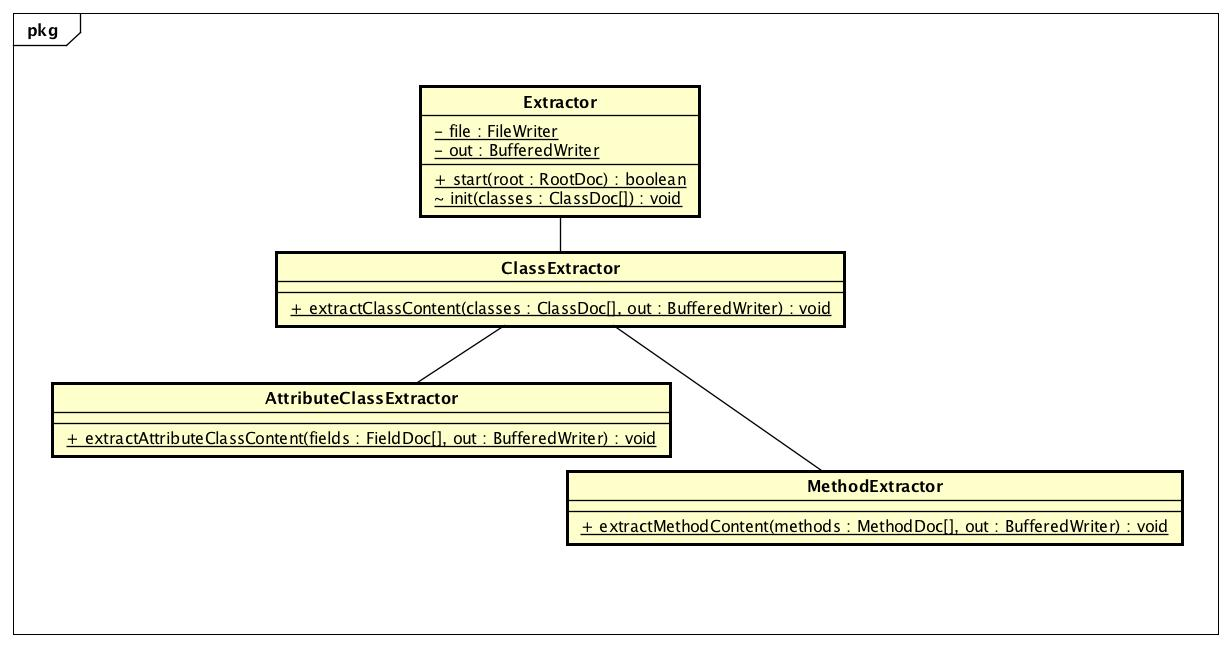
\includegraphics[scale=0.4]{kelas-diagram}  
	\caption[Kelas Diagram]{Kelas Diagram} 
	\label{fig:kelas-diagram} 
\end{figure}

\begin{enumerate}
\item \texttt{Extractor}

Kelas ini merupakan kelas untuk menjalan \textit{custom doclet}

Atribut yang dimiliki kelas ini adalah sebagai berikut.
\begin{itemize}
\item \texttt{String fileName} - atribut untuk nama \textit{file}
\end{itemize}
\textit{Method-method} yang dimiliki kelas ini adalah sebagai berikut.
\begin{itemize}
\item \texttt{public static boolean start(com.sun.javadoc.RootDoc root)}

\textit{Method} ini berperan sebagai \textit{method} untuk menjalankan
 \textit{custom doclet}

\textbf{Parameter:}
\begin{itemize}
\item \texttt{RootDoc root} - 
berperan sebagai mengambil seluruh informasi spesifik dari
             \textit{option} yang terdapat pada \textit{command-line} sebuah
             \textit{terminal}. Selain itu berperan juga untuk mengambil informasi dari
             sekumpulan \textit{file java} yang akan di proses.
\end{itemize}
\textbf{Return Value}: kondisi true

\textbf{Exception}: Tidak memiliki \textit{exception}

\item \texttt{private static void init(com.sun.javadoc.ClassDoc[] classes)}

\textit{Method} ini berperan untuk menulis kedalam sebuah \textit{file}
 saat \textit{javadoc} berjalan.

\textbf{Parameter:}
\begin{itemize}
\item \texttt{ClassDoc[] classes} - 
sebuah array yang berisikan sekumpulan \textit{file java}
                yang akan di proses.
\end{itemize}
\textbf{Return Value}: Tidak memiliki \textit{return value}

\textbf{Exception}: Tidak memiliki \textit{exception}

\item \texttt{public static int optionLength(java.lang.String option)}

Method untuk menghitung banyak option yang digunakan pada
 \textit{command-line}

\textbf{Parameter:}
\begin{itemize}
\item \texttt{String option} - 
sebuah option
\end{itemize}
\textbf{Return Value}: panjang setiap option

\textbf{Exception}: Tidak memiliki \textit{exception}

\item \texttt{public static boolean validOptions(java.lang.String[][] args, com.sun.javadoc.DocErrorReporter err)}

Pengecekan option valid

\textbf{Parameter:}
\begin{itemize}
\item \texttt{String[][] args} - 
String array 2 dimensi dari option
\item \texttt{DocErrorReporter err} - 
sebuah error jika tidak terdapat option tersebut.
\end{itemize}
\textbf{Return Value}: bernilai true jika option tersebut dikenali, false jika option
 tersebut tidak dikenali

\textbf{Exception}: Tidak memiliki \textit{exception}

\end{itemize}
\item \texttt{ClassExtractor}

Kelas ini merupakan kelas untuk mengambil informasi dari sebuah kelas

Kelas ini tidak memiliki atribut. \textit{Method-method} yang dimiliki kelas ini adalah sebagai berikut.
\begin{itemize}
\item \texttt{public static void extractClassContent(com.sun.javadoc.ClassDoc[] classes, java.io.BufferedWriter out)}

\textit{Method} ini akan menampilkan nama kelas berserta penjelasan dari
 sebuah kelas

\textbf{Parameter:}
\begin{itemize}
\item \texttt{ClassDoc[] classes} - 
sebuah array berisikan sejumlah kelas
\item \texttt{BufferedWriter out} - 
turunan dari kelas \texttt{Writer} yang digunakan untuk menulis
                file text
\end{itemize}
\textbf{Return Value}: Tidak memiliki \textit{return value}

\textbf{Exception}: Tidak memiliki \textit{exception}

\end{itemize}
\item \texttt{MethodClassExtractor}

Kelas ini merupakan kelas untuk mengambil informasi sebuah \textit{method}
 terdapat pada kelas

Kelas ini tidak memiliki atribut. \textit{Method-method} yang dimiliki kelas ini adalah sebagai berikut.
\begin{itemize}
\item \texttt{public static void extractMethodClassContent(com.sun.javadoc.ClassDoc superclass, com.sun.javadoc.MethodDoc[] methods, java.io.BufferedWriter out)}

\textit{Method} ini akan menampilkan \textit{method-method} yang dimiliki
 oleh sebuah kelas

\textbf{Parameter:}
\begin{itemize}
\item \texttt{ClassDoc superclass} - 
sebuah objek ClassDoc
\item \texttt{MethodDoc[] methods} - 
sebuah array berisikan sejumlah \textit{method} dari kelas
\item \texttt{BufferedWriter out} - 
turunan dari kelas \texttt{Writer} yang digunakan untuk menulis
                   file text
\end{itemize}
\textbf{Return Value}: Tidak memiliki \textit{return value}

\textbf{Exception}: Tidak memiliki \textit{exception}

\item \texttt{private static void ParameterMethod(java.io.BufferedWriter out, com.sun.javadoc.Parameter[] paramMethod, com.sun.javadoc.ParamTag[] paramTags)}

\textit{Method} ini akan menampilkan parameter \textit{method-method} yang dimiliki
 oleh sebuah kelas

\textbf{Parameter:}
\begin{itemize}
\item \texttt{BufferedWriter out} - 
turunan dari kelas \texttt{Writer} yang digunakan untuk menulis file text
\item \texttt{Parameter[] paramMethod} - 
sebuah array berisikan sejumlah \textit{method} dari kelas
\item \texttt{ParamTag[] paramTags} - 
sebuah array berisikan sejumlah parameter \textit{method} dari kelas
\end{itemize}
\textbf{Return Value}: Tidak memiliki \textit{return value}

\textbf{Exception}: Tidak memiliki \textit{exception}

\item \texttt{private static void ReturnTypeMethod(java.io.BufferedWriter out, com.sun.javadoc.Type type, com.sun.javadoc.Tag[] returnTags)}

\textit{Method} ini akan menampilkan \textit{return type} dari \textit{method-method} yang dimiliki
 oleh sebuah kelas

\textbf{Parameter:}
\begin{itemize}
\item \texttt{BufferedWriter out} - 
turunan dari kelas \texttt{Writer} yang digunakan untuk menulis file text
\item \texttt{Type type} - 
sebuah objek Type
\item \texttt{Tag[] returnTags} - 
sebuah array berisikan sejumlah \textit{return type} dari \textit{method} dari kelas
\end{itemize}
\textbf{Return Value}: Tidak memiliki \textit{return value}

\textbf{Exception}: Tidak memiliki \textit{exception}

\item \texttt{private static void ExceptionMethod(java.io.BufferedWriter out, com.sun.javadoc.Tag[] throwTags)}

\textit{Method} ini akan menampilkan \textit{return type} dari \textit{method-method} yang dimiliki
 oleh sebuah kelas

\textbf{Parameter:}
\begin{itemize}
\item \texttt{BufferedWriter out} - 
turunan dari kelas \texttt{Writer} yang digunakan untuk menulis file text
\item \texttt{Tag[] throwTags} - 
sebuah array berisikan sejumlah \textit{exception} dari \textit{method} dari kelas
\end{itemize}
\textbf{Return Value}: Tidak memiliki \textit{return value}

\textbf{Exception}: Tidak memiliki \textit{exception}

\end{itemize}
\item \texttt{AttributeClassExtractor}

Kelas ini merupakan kelas untuk mengambil informasi sebuah atribut yang
 terdapat pada kelas

Kelas ini tidak memiliki atribut. \textit{Method-method} yang dimiliki kelas ini adalah sebagai berikut.
\begin{itemize}
\item \texttt{public static void extractAttributeClassContent(com.sun.javadoc.FieldDoc[] fields, java.io.BufferedWriter out)}

\textit{Method} ini akan menampilkan atribut-atribut yang dimiliki oleh
 sebuah kelas

\textbf{Parameter:}
\begin{itemize}
\item \texttt{FieldDoc[] fields} - 
sebuah array berisikan sejumlah atribut dari kelas
\item \texttt{BufferedWriter out} - 
turunan dari kelas \texttt{Writer} yang digunakan untuk menulis
 file text
\end{itemize}
\textbf{Return Value}: Tidak memiliki \textit{return value}

\textbf{Exception}: Tidak memiliki \textit{exception}

\end{itemize}
\end{enumerate}

\section{Rancangan Antarmuka}
\label{sec:antarmuka}
Rancangan antarmuka perangkat lunak adalah melalui sebuah {\it Terminal} pada {\it Linux/Mac} atau {\it Command Prompt} pada {\it Windows}. Berikut adalah antarmuka jika menggunakan {\it Terminal} pada {\it Mac}: 

\begin{figure}[H]
	\centering  
	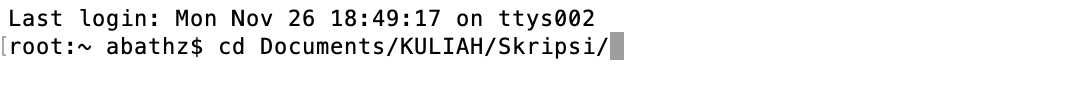
\includegraphics[scale=0.7]{1}  
	\caption[]{Mengarahkan kedalam folder dari perangkat lunak} 
	\label{fig:1} 
\end{figure}
Langkah pertama adalah berpindah dari direktori awal ke direktori perangkat lunak yang dibuat. Untuk berpindah direktori perlukan perintah \texttt{cd} atau kepanjangan dari {\it change directory} lalu diikuti dengan lokasi direktori yang diinginkan. Pada Gambar \ref{fig:1} direktori perangkat lunak terdapat di dalam folder Document lalu folder KULIAH lalu folder Skripsi kemudian tekan tombol {\it enter} lalu direktori akan langsung berpindah ke direktori yang dituju.

\begin{figure}[H]
	\centering  
	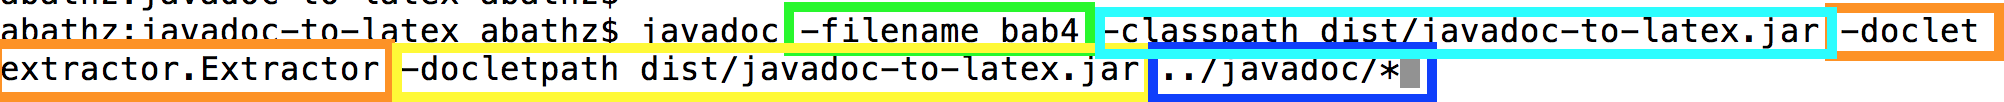
\includegraphics[scale=0.6]{2}  
	\caption[]{Memasukkan perintah yang akan digunakan} 
	\label{fig:2} 
\end{figure}
Langkah kedua adalah menjalan perangkat lunak yang dibuat. Diawali dengan perintah perintah \texttt{javadoc} lalu dikuti 5 buah argumen. Argumen pertama yaitu {\tt -filename} adalah {\it option} untuk menamai {\it file} sesuai dengan yang ditentukan. Sebagai contoh pada Gambar \ref{fig:2}, {\it file} akan bernama "file", jika argumen pertama tidak dimasukkan pada {\it command-line} maka nama dari {\it file} tersebut secara otomatis menjadi "doc". Argumen kedua yaitu {\tt -classpath} berperan sebagai penunjuk kelas-kelas yang digunakan. Argumen kedua ini bersifat {\it optional}, jika kode program yang akan didokumentasikan menggunakan {\it external library} maka argumen ini dibutuhkan. Argumen ketiga yaitu {\tt -doclet} adalah sebuah kelas untuk menjalankan {\it custom doclet} dari perangkat lunak yang dibuat. Argumen ketiga tersebut akan menjalankan kelas bernama \texttt{Extractor} yang terdapat didalam {\it package} \texttt{extractor}. Kemudian argumen keempat yaitu {\tt -docletpath} adalah {\it custom doclet} yang berperan untuk mengambil informasi kelas, atribut, {\it method} dari sekumpulan {\it file java}. Argumen kelima yaitu {\tt -sourcepath} adalah lokasi sekumpulan {\it file java} yang akan diproses. Pada gambar \ref{fig:2}, lokasi {\it file-file} tersebut terdapat pada folder GenerateJavadocToLatex lalu folder {\it src} lalu argumen keenam yaitu adalah sebuah {\it package} yang berisikan sekumpulan {\it file Java}, pada kasus ini adalah {\it package extractor}.

\begin{figure}[H]
	\centering  
	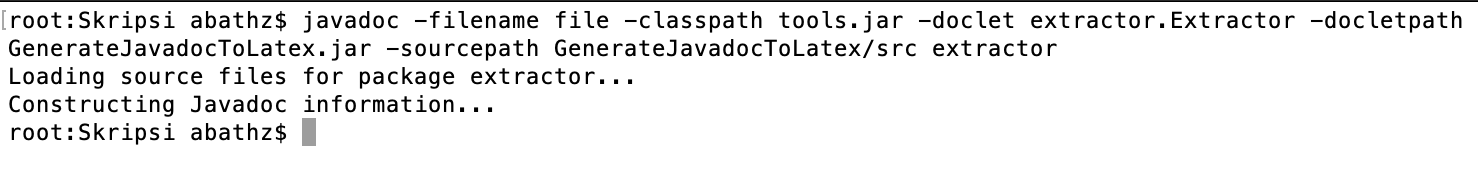
\includegraphics[scale=0.6]{3}  
	\caption[]{Hasil tampilan jika proses konversi selesai} 
	\label{fig:3} 
\end{figure}
Perangkat lunak yang dibuat akan membaca seluruh isi {\it package}. Pada contoh Gambar \ref{fig:3}, perangkat lunak akan melakukan pengambilan informasi terhadap {\it package} tersebut. Jika proses pengambilan selesai maka proses berhenti.
























